\startchapter{A kinetic model and API of PDI}

\section*{Introduction}

\subsection*{Antibiotic resistance}
Antibiotic resistant infections are projected to exceed cancer in annual deaths, and globally cost $10^{13}~USD$ in lost economic production, by mid-21st century \cite{ONeill2014AntimicrobialNations}. Meticillin-resistant \textit{Staphylococcus aureus} (MRSA) and fluoroquinolone-resistant \textit{Salmonella} \cite{Moghnieh2018EpidemiologyLeague} are two worrisome examples of virulent pathogens that are developing resistance to the antimicrobial treatments that subdued them during the 20th century  \cite{Theuretzbacher2013GlobalStory,Levy2004AntibacterialResponses,Wyles2017Post-treatmentLedipasvir/sofosbuvir,Nowak1997Anti-viralPopulations}. Bacterial colonies (biofilms) -- which cause persistent infections \cite{Metcalf2013BiofilmEvidence} and degrade industrial surfaces  \cite{Matin2011BiofoulingPrevention} and polymers \cite{Cantor1969BiologicalMembranes,Murphy2001MicrobiologicalMembranes} in a process called biofouling, such as water filtration membranes \cite{Ivnitsky2005CharacterizationTreatment,Herzberg2007BiofoulingPressure,Schneider2005DynamicsBiofouling} and boat hulls \cite{Schultz2011EconomicShip} -- are moreover exceptionally resilient to conventional antimicrobial treatments \cite{Jamal2018BacterialInfections,Singhai2012AResistance}. This resilience extends from the metabolic capacity of biofilm communities often neutralizing \cite{Pereira2011SusceptibilityStudy}, and the extracellular polymeric substances (EPS) of the biofilm matrix limiting the diffusion of \cite{Suci1994InvestigationBiofilms,Hoyle1992PseudomonasPiperacillin,LeChevallier1988InactivationBacteria,Dunne1993DiffusionBiofilm}, antimicrobial agents. 

Antimicrobial resistance, particularly with planktonic organisms, is the manifestation of a few factors: 1) the excessive and incomplete use of antibiotics for illness; 2) runoff from animal agriculture, which is globally the primary consumer of antibiotics \cite{VanBoeckel2017ReducingAnimals,Eggleton2020TheWorld}; and 3) highly specific biochemical targets of the antimicrobial agents, which place selective evolutionary pressure on the pathogen to fortify its targeted vulnerabilities. The first two causes are the consequence of social norms and practices, and thus are better solved through activism, while the third cause is biological and thus can resolved by replacing the contemporary medical arms race of chemists against evolution with a more efficient and sustainable medical strategy, and one that ideally also avoids the persist ecotoxicity that is observed with conventional organic antibiotics \cite{Thomas2001AntifoulingEffects,Niu2016RolesIrradiation,Winters1983ControlDesalination}.

\subsection*{Photodynamic inactivation}

Photodynamic inactivation (PDI), which is mechanistically synonymous with photodynamic therapy (PDT) for cancer treatment \cite{Lange2019ComparisonLines}, offers an new strategy for treating prokaryotic \cite{Hamblin2004PhotodynamicDisease,Lange2019ComparisonLines} and viral \cite{Wigginton2010OxidationInactivation,Lebedeva2020TheViruses} pathogens. PDI describes a photochemical process of non-selectively oxidizing biological substrate \cite{Choe2006MechanismsOxidation,Frankel1980LipidOxidation} with reactive oxygen species (ROSs) \cite{Zepp1992HydroxylReaction,Koppenol2001TheLater}. The primary ROS from PDI is singlet state oxygen ($\ce{^1O2}$) \cite{Ergaieg2008InvolvementPorphyrin, Allen2004IntroductionSimulations, Henze2019Multi-scaleCheckpoint, Zaman2005ComputationalMatrices,Gillespie2007StochasticKinetics}, which is the lowest excitation state of diatomic oxygen, whose ground conformation is a triplet state ($\ce{^3O2^.}$). This mechanism enables PDI to simultaneously 1) avoid resistance evolution \cite{Tavares2010AntimicrobialTreatment,Lauro2002PhotoinactivationConjugates,Pedigo2009AbsenceTherapy}; 2) treat recalcitrant biofilms \cite{Beirao2014PhotodynamicPorphyrin,Ghorbanzadeh2020ModulationModel}, where the biofilm matrix is itself oxidized by $\ce{^1O2}$; and 3) avoid ecological presistence, since $\ce{^1O2}$ has only a $\approx 100 nm$ diffusion distance and a $\approx 10^{-6} s$ lifetime \cite{Moan1984TheOxygen, Moan1990OnTissues,Rodgers1982LifetimeMeasurements}. The latter quality encourages the use of PDI in wastewater treatment \cite{Kohn2007AssociationOxygen,Mostafa2013SingletMatter,Jimenez-Hernandez2006SolarSensitizers} and surfaces \cite{McCoy2014PhotodynamicControl} or industrial polymers \cite{Kim2003DesignProblem} where the antimicrobial agent won't leach into the environment or human consumables. 

The singlet and triplet electronic states that are mechanistically involved in PDI are defined by their quantum multiplicity. The molecular singlet state contains only paired electrons and is named after its multiplicity of $1$: from $2(S)+1=1$, where $S$ (the total molecular angular momentum, which is the sum of each up electron spin as $+\frac{1}{2}$ and each down electron spin as $-\frac{1}{2}$) equates 0 since the quantities of up and down electrons are necessarily equivalent (Figure S1). The molecular triplet state, in contrast, contains two unpaired (radical) electrons and is defined by a multiplicity of $3$: from $2(S)+1=3$, where $S=1$. These unpaired electrons in $\ce{^3O2^.}$ minimize electrical shielding of the nuclear charge \cite{Katriel1972ARule} and consequently stabilize $\ce{^3O2^.}$ by $0.98$ eV \cite{Jockusch2008SingletExcitation} relative to $\ce{^1O2}$ that contains additional nuclear shielding.

A photosensitizer catalyst (PS) is essential to generate antimicrobial concentrations of $\ce{^1O2}$. This is the consequence of the direct excitation $\ce{^3O2^. ->[{hv}] ^1O2}$ \cite{Krasnovsky2012PhotochemicalEnvironment} being unlikely and technically forbidden by the formal selection rules of electronic excitation\cite{Bowen1936ForbiddenLines}, where the most probable excitations are those that preserve the molecular electronic state, instead of transitioning from triplet to singlet. The $\ce{^3O2^.}$ could potentially excite to a triplet state and then relax into $\ce{^1O2}$ \cite{Long2003SelectionOxygen}; nevertheless, the PS catalyst accelerates $\ce{^3O2^.}$ excitation through energy transfers \cite{You2018ChemicalOxygen,Schalk2008Near-infraredTetratolyl-porphyrins,Jockusch2008SingletExcitation}, and moreover introduces desirable control over localizing $\ce{^1O2}$ within a system by selectively placing the PS in the desired location.

PDI with $\ce{^1O2}$ generally acts through Type II oxidation mechanisms, which are concerted Schenck \cite{Prein1996TheApplications} or Alder-ene \cite{Fernandez-torquemada2012DispersionPlants} reactions that produce organic peroxides \cite{Foote1965ChemistrySelectivity}, as opposed to Type I mechanisms \cite{Bolland1949KineticsOxidation,Farmer1943TheRubber,Grynova2011RevisingAutooxidation} that only affect radical substrates \cite{Litwinienko1999DifferentialEsters}. This Type II mechanism most readily affects allylic positions of unsaturated molecules \cite{Ellison1996ThermochemistryIons,Sehon1950TheRadical}, although, saturated molecules are also oxidized by $\ce{^1O2}$. The first mechanistic step of PDI describes the ground-state ($\ce{^1PS}$) absorbing a photon ($hv$) and entering an excited singlet state ($\ce{^1PS^*}$), according to the selection rules of excitation. This excited state then relaxes through intersystem crossing, instead of fluorescing \cite{Kessel1982DeterminantsSpectra}, to an excited triplet state ($\ce{^3PS^.}$),
\begin{equation} \label{ps_excitation_steps}
    \ce{^1PS <=>[{excitation}][{fluorescence}] ^1PS^* ->[][{intersystem-crossing}] ^3PS^.}~.
\end{equation}
The $\ce{^3PS^.}$ then relays the excitation energy to $\ce{^3O2^.}$, instead of phosphorescing \cite{Mcrae1958Enhancement6}, and thereby regenerates the ground-state $\ce{^1PS}$ while generating $\ce{^1O2}$,
\begin{equation} \label{excited_ps_steps}
    \ce{^1 PS <-[{phosphorescence}] ^3 PS^. + ^3O2^. &-> ^1 PS + ^1O2}
\end{equation}
The efficiency of this excitation mechanism is encapsulated in a quantum yield \cite{Bakalova2004QuantumPhotosensitizers} ($0\le \Phi_{\ce{^1O2}}\le 1 ~;~ \frac{\ce{^1O2} ~molecules ~produced}{photon ~absorbed}$). The $\ce{^3PS^.}$ and $\ce{^1O2}$ excited states are more mechanistically involved than $\ce{^1PS^*}$ and $\ce{^3O2^*}$ since fluorescence is more favorable than phosphorescence, according to the selection rules, and thus the former molecules have longer lifetime than the latter molecules. 

\begin{figure}[t]
    \centering
    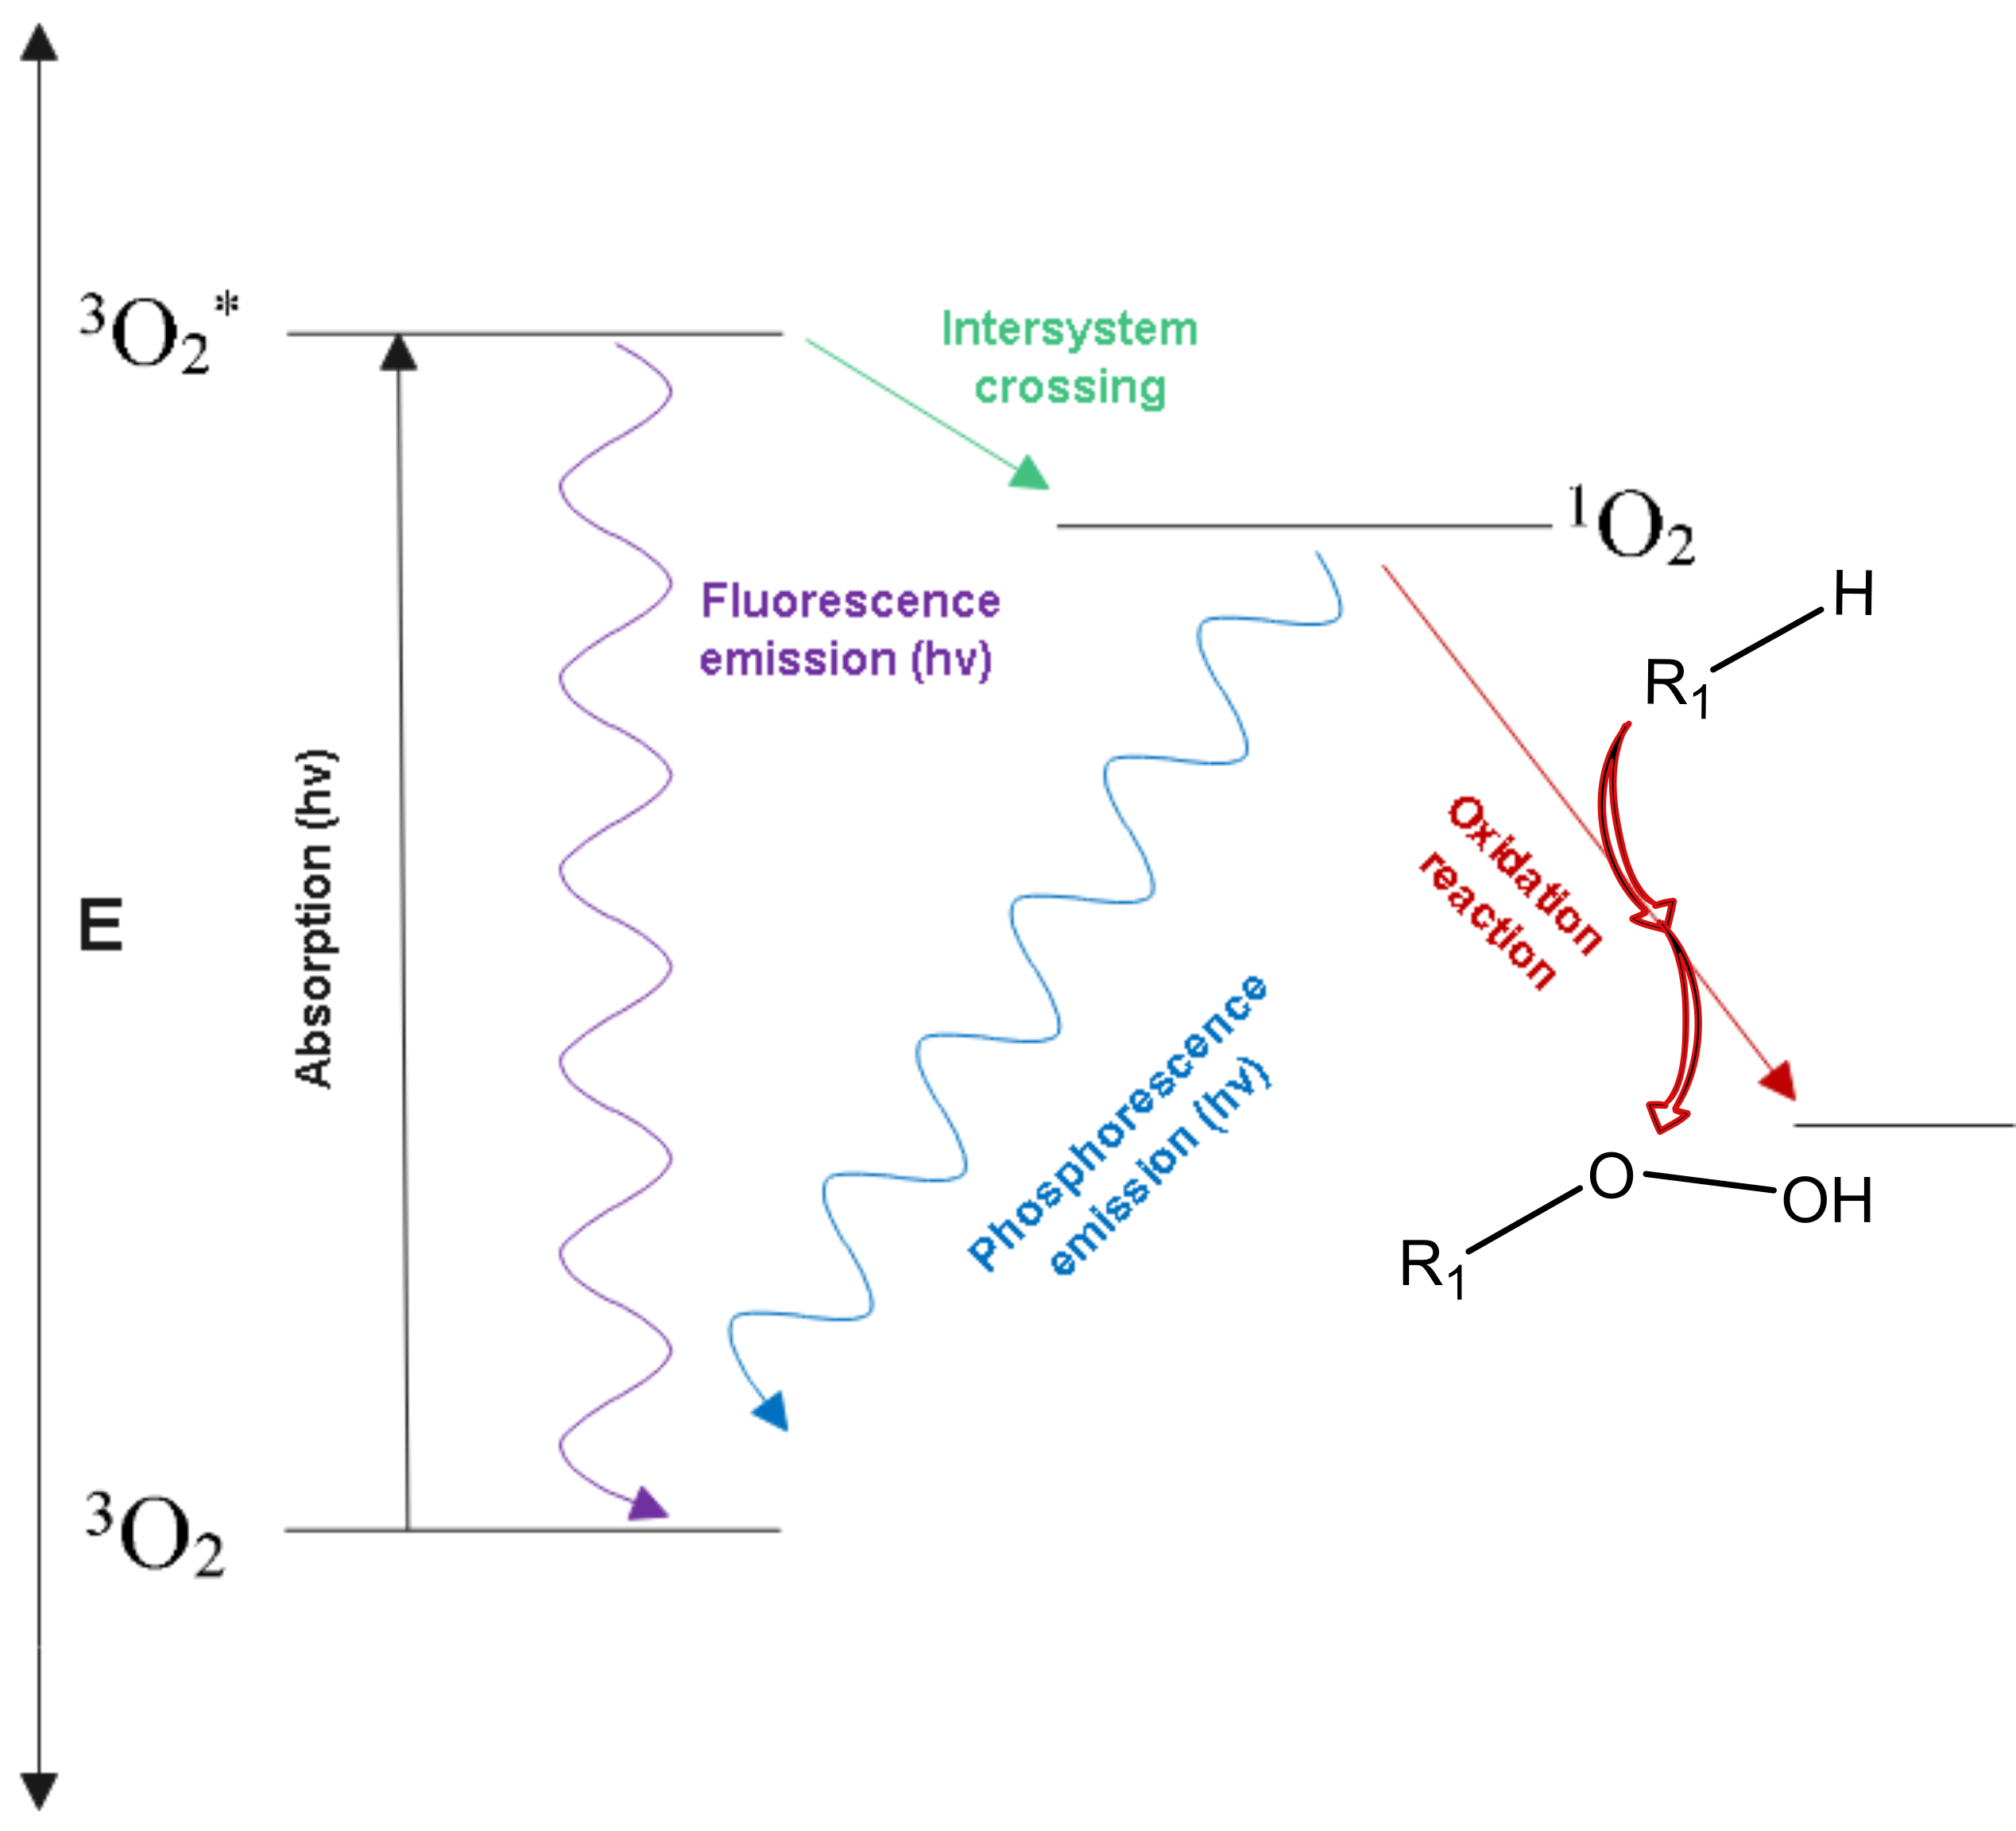
\includegraphics[width = \textwidth]{images/PDIpy/jablonski_diagram.png}
    \caption{
        A qualitative Jablonski energy diagram of photosensitization. The initial electronic absorption of a photon ($h\nu$) by $\ce{^3O2^.}$ forms a $\ce{^3O2^.}$* molecule, following the selection rules of excitation, which is followed with either fluorescence relaxation or an intersystem-crossing relaxation to form the reactive $\ce{^1O2}$. The singlet $\ce{^1O2}$ molecule either relaxes through phosphorescence or it reacts with an organic substrate to form a peroxide, like the illustrated hydroperoxide with a generic “R” organic group. 
    }
    \label{jablonski_diagram}
\end{figure}

\subsubsection*{Photosensitizer}
The efficacy of PDI and $\ce{^1O2}$ production is primarily dependent upon the chemical structure of the photosensitizer catalyst (PS), notwithstanding minor influence of the chemical conditions \cite{Kruk1998PhotophysicsLuminescence,Kullmann2012UltrafastBisporphyrin}. The PS must optimize the $\Phi_{\ce{^1O2}}$ by minimizing fluorescence or phosphorescence, which is depicted in \cref{ps_excitation_steps,excited_ps_steps} and Figure \ref{jablonski_diagram}, and by minimizing the gradual loss of absorptivity from photobleaching, where irradiation irreversibly compromises molecular absorptivity \cite{Bonnett2010ChemInformTherapy,Wasser1973TheMetallochlorins}. The functionality and charge of the PS should furthermore optimize the association of the PS with the targeted cells \cite{VanDerWal1997DeterminationBacteria,Dickson1989CellSurfaces} -- and minimize off-target oxidation \cite{Lambrechts2005PhotodynamicMice} and host toxicities \cite{Quishida2016PhotodynamicLight} in medical applications. Material applications of PDI \cite{Peddinti2018PhotodynamicThreat,Gottenbos2001AntimicrobialBacteria}, for either biofouling or sterile medical surfaces, further require that the PS is amenable to permanent attachment in a manner that retains material properties \cite{McCoy2014PhotodynamicControl}. 

The PS finally influences the biological targets of PDI. Impermeable PSs cannot penetrate a cell and thus generally oxidize the cytoplasmic membrane \cite{Specht1990DepolarizationAction,Ehrenberg1993ElectricAlterations} instead of cytoplasmic contents \cite{Maisch2004AntibacterialDermatology}. This mechanism, which primarily affects the phospholipid fatty acids in Figure \ref{schenck_mechanism}, manifests in cell death through lysis \cite{Sahu2009AtomicColi,Bertoloni1987RoleCells}, and affects gram-positive bacteria more than gram-negative bacteria \cite{Lauro2002PhotoinactivationConjugates,Merchat1996Meso-substitutedBacteria} since the latter possesses a superficial lipopolysaccharide layer that protects the cytoplasmic membrane. Permeable PSs, by contrast, can penetrate a cell and thus generate $\ce{^1O2}$ within the cytoplasm where cytoplasmic chemicals \cite{Bagchi1979RoleAcriflavine} such as guanine nucleotides \cite{Prat1997Determination9,Devasagayam1991FormationOxygen} are fatally oxidized. This mechanism is more effective with prokaryotes than eukaryotes \cite{Quishida2016PhotodynamicLight}, since the latter have nuclear membrane that protect DNA, particularly guanine, from oxidation \cite{Pereira2013PhotodynamicVitro}.

A narrow range of chemicals meet these criteria of an ideal PS. Semiconductors \cite{Nelson2002PhotoconductivityDioxide,Peiro2006PhotochemicalPreparations,Linsebigler1995PhotocatalysisResults}, and some amino acid residues \cite{Lippincott-schwartz2003PhotobleachingTechniques,Jin1995PhotolysisSolution}, can electrocatalytically generate $\ce{^1O2}$; however, these molecules are inefficient and/or impractical, particularly for medical applications. The most efficacious PS in nature is chlorophyll \cite{Ramel2012ChemicalPlants}, which is an organometallic porphyrinoid that evolution has tuned for visible light -- specifically blue-violet radiation \cite{Mtangi2017ControlSplitting} through the Soret band \cite{Carre1999FungicidalCerevisiae,Pereira2014InfluencePorphyrin,Ashkenazi2003PhotodynamicBacteria,Moan1986PorphyrinShGroups,Nitzan1992InactivationPorphyrins,Durantini2006PhotodynamicBacteria,Salmon-Divon2004MechanisticTetra-mesoN-methylpyridylporphine} and green-orange radiation \cite{Bertoloni2000PhotosensitizingCells} through the Q band \cite{Bonnett1999PhotobleachingStudy,Jori2006PhotodynamicApplications,Gad2004TargetedMice,Zhao2019Porphyrin-basedAbsorption} -- and low rates of photobleaching. Chlorophyll, however, has not evolved traits that optimize its association with cellular targets or its compatibility with material surfaces; therefore, synthetic porphyrins \cite{Orenstein1997TheInfections,Beirao2014PhotodynamicPorphyrin,Merchat1996StudiesPorphyrins} that emulate the successful conjugated structure \cite{Huang2008Porphyrin-dithienothiopheneCells} of chlorophyll, while introducing other metal centers \cite{Mosinger1997QuantumPorphine} and functional handles  \cite{Hirao1999TheoreticalDerivatives,Wu2014BODIPY-basedSolution,Chacon1988SingletArachidonic} that improve its utility in PDI \cite{Jager2016QScales,Karolczak2004PhotophysicalTetraphenylporphyrin,Mathai2007SingletTherapy}, is an appealing direction for PDI research. 

\begin{figure}[t]
    \centering
    \includegraphics[width = \textwidth]{images/PDIpy/BCFA_schenck_oxidation_2.png}
    \caption{
         The Schenck reaction and associated byproduct decompositions. Step (1) depicts the concerted\cite{Foote1968PhotosensitizedOxygen} Schenck reaction. Step (2) depicts the homolytic cleavage of the hydroperoxide bond to form $\ce{OH^.}$ and an oxy radical that may enter autoxidation mechanisms. Step (3) depicts radical propagation via hydrogen abstraction to form another radical substrate and an alcohol byproduct as part of the autoxidation mechanism. Step (4) is a concerted Russell reaction\cite{Russell1957Deuterium-isotopeRadicals,Howard1968TheMechanism} between two hydroperoxides that forms a $\ce{H2O2}$, an $\alpha,\beta$-ketone, and an alcohol. The reactions of Steps (2-4) sample the wide array of possible oxidative decompositions that follow the Schenck or autoxidation mechanisms.
    }
    \label{schenck_mechanism}
\end{figure}

\subsection*{PDI modeling}
Computational models of PDI that allow experimentalists, biologists and chemists alike, to explore the efficacies of different PSs, based upon their characteristics, and system conditions are scarce. Santos et al. \cite{Santos2020ApplicationAureus} developed a second-order polynomial to mathematically describe the inactivation of \textit{S. aureus} as a function of time at a particular wavelength and PS concentration. The predictions were demonstrated to be accurate, however, the model is bound to a narrow range of conditions, and does permit the investigator to explore parameters such as PS characteristics. Brasel et al. \cite{Brasel2020AnAgalactiae} developed a logistic model to assess the sensitivity of PDI inactivation to incident irradiance. This interestingly revealed that only the total incident exposure $\frac{J}{cm^2}$, and not the rate of exposure as irradiance $\frac{mW}{cm^2}$, is consequential for bacterial inactivation; however, the model likewise does not permit investigations of alternative PDI systems, and thus the model is minimally applicable for experimentalists. Sabino et al. \cite{Sabino2019InactivationTherapy} developed a Weibull power-law function from fitted inactivation data to predict lethal doses and the tolerance factor of a PDI system; yet, the model is confined to an excel spreadsheet, and thus is not amenable to the workflows that are used by computational biologists. 

We therefore developed a kinetic model of PDI that improves the mechanistic resolution of PDI relative to existing models, and we further encapsulated this model into a comprehensive API (PDIpy), which allows investigators to efficiently explore a continuum of values for numerous parameters. PDIpy uses Tellurium \cite{Choi2018Tellurium:Biology} to concisely construct SBML \cite{Keating2020Models}, SED-ML \cite{Waltemath2011ReproducibleLanguage}, and COMBINE OMEX \cite{Bergmann2014COMBINEProject} descriptions of the simulations and their results, which are conventions that supports reproducibility of biological simulations. We exemplify the kinetic model and PDIpy through replicating experimental studies and a few sensitivity analyses. We expect that the open-source project will allow experimentalists to rapidly assess experimental designs without expending resources, and will inspire computational biologists to refine tools for this field of medical research, towards expediting the scientific response to the looming medical crisis of antibiotic resistance. 

\section*{Methods}
\subsection*{Conceptual model}
PDIpy conceptually represents an experimental PDI system with an impermeable PS and a cocci bacterium like \textit{S. aureus}. Each simulation therefore requires details about the light conditions (e.g. the light source and the incident intensity), the microbial conditions (e.g. the bacterial specie and the $\frac{CFU}{mL}$ for planktonic experiments), and the photosensitizer characteristics (e.g. the PS structure and the $\frac{mol}{vol}$ or $\frac{mol}{area}$ concentration of the photosensitizer). Default parameters in each of these categories can supplement user-defined parameters. 

\subsection*{Kinetic reactions}
The PDI model is predicated upon a set of kinetic reactions that represent the essential processes of PDI. 1) The first reaction describes the photoelectric effect \cite{Wheaton2009PhotoelectricEffect} after $\ce{^1PS}$ is struck by a photon ($hv$) to form $\ce{^3PS^.}$, which is depicted in \cref{ps_excitation_steps}. A detrimental alternative reaction is photobleaching, where the absorptive ability of PS is irreversibly compromised by photonic collision. 2) The second major reaction describes an energy transfer from $\ce{^3PS^.}$ to $\ce{^3O2^.}$, which is depicted in \cref{excited_ps_steps}. 3) The third major reaction describes $\ce{^1O2}$ oxidizing biological substrates, which includes both cytoplasmic phosholipids and biofilm polymeric substances, depending upon the simulation specifications. Each of these aforementioned PDI reactions are detailed in the following sub-sections.

\subsubsection*{Photoelectric}
\paragraph{PS excitation}
PDI begins with excitation of the PS in \cref{ps_excitation_steps}, which is represented through the kinetic expression
\begin{multline} \label{ps_excitation_kinetics}
    \frac{d[\ce{^3PS^.}]}{dt} =  k_{excitation}*\frac{photons_{PS}}{photons_{total}} \\ 
    *\Phi_{excitation}*[\ce{^1PS}] - k_{fluorescence}*[\ce{^3PS^.}]. 
\end{multline}
The $k_{excitation}$ \& $k_{fluorescence}$ rate constants are estimated as the inverse of the rise and decay times for the PS, respectively, which depend upon the selected photosensitizer. The approximate rise time for a porphyrin PS is $50 fs$, which is consistent with estimates of $<100 fs$ \cite{Andersson1999PhotoinducedState} and $60-90 fs$ in ethanol solvent \cite{Gurzadyan1998Time-resolvedZn-tetraphenylporphyrin}. The approximate decay time for a porphyrin PS is $1.5 ns$ for the S2 fluorescence \cite{Akimoto1999UltrafastPorphyrins}. The $\Phi_{excitation}$ ($\frac{PS excited}{photon absorbed}$) is likewise a property of the photosensitizer and is $\approx 0.7$ for porphyrins \cite{Krasnovsky2012PhotochemicalEnvironment}. The $\frac{photons_{incident}}{photons_{total}}$ \cite{Brasel2020AnAgalactiae}, which is the proportion of incident photons that strike a photosensitizer in the system, is calculated through a series of steps. First, the reported intensity of incident light from the respective light source -- i.e. either irradiance ($\frac{mW}{cm^2}$), exposure ($\frac{J}{cm^2}$), lux ($\frac{lumen}{m^2}$), or lumens (lumens) -- is converted into $watts_{emitted}$ ($\frac{J}{s}$). Second, this wattage is attenuated by the proportion of the emission spectrum $light_{emitted}$ that resides within the excitation spectrum of the photosensitizer $light_{excitation}$,
\begin{equation}
    watt_{excitation} = \frac{light_{excitation}}{light_{emitted}}*watts_{emitted}.
\end{equation}
Third, the $watt_{excitation}$ is used to calculate the moles of incident photons that strike photosensitizers per timestep 
\begin{multline} \label{photons_per_second}
    \frac{photons_{PS}}{timestep}=\frac{<h\nu_{excitation}>}{h*c}*watts_{excitation} \\
    *\frac{second}{timestep}*reflection*\frac{1 mole}{N_A}*\frac{vol_{PS}}{vol_{total}},
\end{multline}
where $reflection$, which represents proportion of incident photons that penetrate an aqueous solution versus being reflected, is estimated as $96 \%$ \cite{Gross1993SingletLiposomes}; the $\frac{vol_{PS}}{vol_{total}}$ represents the proportion of volume of all PSs in the solution ($vol_{PS}$) -- which is the product of the quantity of PS molecules and the volume per molecule that is calculated through trigonometry of the molecular structure -- to the volume of the solution in which the PS resides $vol_{total}$ \cite{Santos2020ApplicationAureus}; and the average excitation wavelength of the PS ($<h\nu_{excitation}>$) is calculated as the weighted average of the Soret and Q excitation bands, in proportion to their relative contribution in generating $\ce{^1O2}$ \cite{Nitzan2001PhotoinactivationWavelengths,Hoenes2020PhotoinactivationWavelength}. The resultant $\frac{photons_{PS}}{timestep}$ from \cref{photons_per_second} is then divided by the $\frac{photons_{total}}{timestep}$ to complete the kinetic expression in \cref{ps_excitation_kinetics} that calculates the excitation of PS in each timestep. 

\paragraph{Photobleaching}
The collision of a PS and a photon may alternatively disrupt the conjugated PS system, and prevent further excitation through the irreversible reaction of photobleaching
\begin{equation} \label{bleaching}
    \ce{^1PS -> ^1PS_{bleached}}
\end{equation}
and the corresponding kinetic expression
\begin{equation} \label{bleaching_kinetics}
    \frac{d[\ce{^1PS_{bleached}}]}{dt} = k_{bleaching}*[\ce{^1PS}].
\end{equation}
The $k_{bleaching}$ rate constant varies with the chemical structure of the PS, although, it is reported for porphyrins to be within the range $[1.5E-4, 4E-2] \frac{cm^2}{W}$ for the oxygen-independent, first-order, reaction \cite{Bonnett1999PhotobleachingStudy, Dysart2005CalculationCells, Mang1987PhotobleachingTherapy}, as opposed to oxygen-dependent photobleaching that is observed \textit{in vivo} \cite{Dysart2005CalculationCells}. The rate constant is a function of light exposure $\frac{J}{cm^2}$ for the PDI system.

\subsubsection*{Energy Transfer}
The energy transfer from $\ce{^3PS^.}$ to $\ce{^3O2^.}$  in \cref{excited_ps_steps} is described with an associated kinetics expression
\begin{equation} \label{energy_transfer_kinetics}
    \frac{d[\ce{^1O2}]}{dt} = k_{transfer}*\Phi_{transfer}*[^3PS]*[\ce{^3O2^.}]. 
\end{equation}
The rate constant $k_{transfer}$ is the inverse of the decay time of $\ce{^3PS^.}$, which for a porphyrin PS appears to be $100 ns$ in aqueous after accounting for the use of acetone media, which significantly increases the lifetime of excited states \cite{Spikes1992QuantumUroporphyrin}, in the reported $\approx 200 ns$ \cite{Kupper2002KineticsOxygen} value. The $\ce{^1O2}$ phosphorescence side reaction, which often emits a specific infrared wavelength that can approximate the $[\ce{^1O2}]$ within the system \cite{Macpherson1993DirectCentres}, is kinetically represented 
\begin{equation}
    \frac{d[\ce{^3O2^.}]}{dt} = k_{phosphorescence}*[\ce{^1O2}]
\end{equation}
where $k_{phosphorescence}$ is approximated with a slope of $\frac{\ce{^1O2}~lifetime}{CFU/mL}$, since the $\ce{^1O2}$ lifetime is greater in biological material and thus is proportional with the bacterial concentration in planktonic simulations \cite{Maisch2007TheBacteria}. The minimum lifetime is constrained to $3.5\mu s$ as a baseline lifetime in pure water \cite{Baier2005Time-resolvedCells}.

\subsubsection*{Oxidation}

\paragraph{Cytoplasmic membrane} 
The oxidation of cytoplasmic phospholipids is represented as an irreversible second-order reaction \cite{Watabe2007OxidationMembranes.}
\begin{equation} \label{membrane_oxidation}
    \ce{^1O2 + FA -> oFA}.
\end{equation}
with an associated second-order kinetic expression
\begin{equation} \label{membrane_oxidation_kinetics}
    \frac{d[oFA]}{dt} = k_{fa}*[\ce{^1O2}]*[FA],
\end{equation}
where the rate constant $k_{fa} \approx 100 \frac{L}{g*s}$ and the phospholipid concentration in the cytoplasmic membrane is described in $\frac{g}{L}$. This rate constant derives from a reported range of $[277,769] \frac{L}{g*s}$ for Type II oxidation of unsaturated fatty acids \cite{Mukai2019KineticSolution}, which are more prone to oxidation and thus the corresponding oxidation rate for saturated fatty acids is lower than the reported values. 

\paragraph{Biofilm matrix} 
The oxidation of EPS is reported to be significant during PDI \cite{Beirao2014PhotodynamicPorphyrin}. This process is represented through an irreversible reaction
\begin{equation} \label{EPS_oxidation}
    \ce{^1O2 + EPS -> oEPS},
\end{equation}
which competes with \cref{membrane_oxidation} for $\ce{^1O2}$ and thereby lessens the efficacy of PDI upon biofilms relative to planktonic organisms. The oxidation of bioiflm polymers is kinetically represented  
\begin{equation} \label{EPS_oxidation_kinetics}
    \frac{d[oEPS]}{dt} = k_{EPS_{oxidation}}*[\ce{^1O2}]
\end{equation}
with an empirical rate constant, which may vary with the simulated specie, and an initial concentration of EPS that is $9x$ greater than the cellular mass, in proportion to mass distributions of biofilms \cite{Flemming2010TheMatrix}.

\subsubsection*{Complete kinetic system}
The amalgamation of the aforementioned kinetic expressions, which constitute the heart of our PDI model, are summarized here:
\begin{align*}
    \ce{^1PS &<=> ^3PS^.} \\
    \ce{^1PS &-> ^1PS_{bleached}} \\
    \ce{^3PS^. + ^3O2^. &-> ^1PS + ^1O2} \\
    \ce{^1O2 &-> ^3O2^.} \\
    \ce{^1O2 + FA &-> oFA} \\
    \ce{^1O2 + EPS &-> oEPS} \\
\end{align*}

\subsection*{Data Processing}

\subsubsection*{Inactivation}
Simulation data of chemical concentrations is processed into predictions of bacterial inactivation. This occurs through first fitting the proportion of oxidized substrate from the data
\begin{equation} \label{oxidation_proportion}
    ox_{proportion} = \frac{[oFA]}{[oFA]+[FA]}
\end{equation}
with a variation of the Hill-equation \cite{Gesztelyi2012ThePharmacology}, which is a biochemical kinetic model that derives from mass-action kinetics, similar to the Michaelis-Menten kinetic model. This variation of the Hill equation \cite{Inoue2016OscillationActivation} introduces an additional "bottom" parameter 
\begin{equation}
    y=bottom+\frac{(top-bottom)*x^n}{EC50^n+x^n}
\end{equation}
that allows for finer control of the plot. The parameters from the fitted regression of the Hill-equation, via the HillFit Python module, are then systematically adjusted to construct an inactivation plot that follows observed results. These adjustments differ for simulations of planktonic versus biofilm bacteria, since biofilms introduce other factors such as impaired diffusion that are not explicitly accounted in our kinetic model. The log-inactivation predictions are generally 1-2 greater than the log-oxidation from \cref{oxidation_proportion}, which embodies our assumption that the membrane lipids of the cell must experience $1-10\%$ oxidation for the cell to die through lysis. Experimental literature has not been discovered to validate this assumption.

% \subsubsection*{Cross-linked systems}

% \paragraph{iPDIpy}
% The PDIpy API is graphically interactive through a user interface iPDIpy, which is depicted in Figure \ref{}. This interface provides a convenient means for parameterizing a PDIpy simulation, exporting and importing sets of parameters, parsing the processed simulation data, viewing error messages and calculated values, viewing the output figure of bacterial reduction over time, and parsing the processed data through a build-in function. The iPDIpy version of PDIpy is downloadable from our GitHub repository.

% \begin{figure}
%     \centering
%     \includegraphics{}
%     \caption{
%         The left pane of the GUI will contain command buttons like restarting the simulation or export results, while the right pane will edit the simulation data and or bacterial qualities/species.
%     }
%     \label{iPDIpy_interface}
% \end{figure}


%%%%%%%%%%%%%%%% Examples %%%%%%%%%%%%%%%%%%%%
% \begin{tablenotes}
% \item[a] This is a table note.
% \item[b] This is another table note.
% \end{tablenotes}

% \end{threeparttable}
% \end{table}

% Let $X_1, X_2, \ldots, X_n$ be a sequence of independent and identically distributed random variables with $\text{E}[X_i] = \mu$ and $\text{Var}[X_i] = \sigma^2 < \infty$, and let
% \begin{equation}
% S_n = \frac{X_1 + X_2 + \cdots + X_n}{n}
%       = \frac{1}{n}\sum_{i}^{n} X_i
% \end{equation}
% denote their mean. Then as $n$ approaches infinity, the random variables $\sqrt{n}(S_n - \mu)$ converge in distribution to a normal $\mathcal{N}(0, \sigma^2)$. Thus concludes the explanation about Eq.~\ref{eq:CLT}.

%%%%%%%%%%%%%%%% Examples %%%%%%%%%%%%%%%%%%%%


\section*{Case Studies}

\subsection*{Cross-linked PS}
Experimental data from our lab with cross-linked PSs (unpublished) was parameterized, in Table \ref{}, into PDIpy. The predicted reduction curve over time in Figure \ref{} agreed with the experimental data at the measured time of 6 hours and 98\% reduction, which supports that the software yields accurate predictions. 

\paragraph{}
.

\paragraph{}
.

\paragraph{}
.

\paragraph{}
.

\subsection*{Solution PS}

\paragraph{Beirao et al.\cite{Beirao2014PhotodynamicPorphyrin}}
This paper experimentally examines a dissolved PS with both planktonic and sessile \textit{S. aureus} (a model cocci organism) and various PS concentrations. 

\paragraph{}
. 

\paragraph{}
.

\section*{Discussion}
The predictions of bacterial reduction from PDIpy appears to be accurate. 

The plateaued response after extended exposure may reflect the presence of dormant persister cells that traditionally evade antimicrobial treatments \cite{Lewis2010PersisterCells,Keren2004PersisterAntimicrobials}

The model assumes that cellular lysis is directly caused by phospholipid oxidation, and that the inactivation rate is experiences a diminishing correlation with the proportion of phospholipid oxidation over time, which further assumes that the membrane chemicals are relatively fixed in the membrane.

\section*{Conclusion}
PDI may effectively modeled through a simple system of chemical kinetics. The open-source implementation of this model through the PDIpy API may both practically support the experimentalists as they develop PDI technologies, and it may ideally inspire other computational biologists to develop programs that can foster discovery in this important niche of antibiotic methods.   


\section*{Author Contributions}
\begin{description}
    \item[APF] Designed, executed, and codified the project.
    % \item[ESC] Contributed the iPDIpy design.
    \item[JRK] Guidance and manuscript edits.
    \item[HLB] Guidance, manuscript edits, and funding.
\end{description}


\section*{Acknowledgments}

The authors are grateful to Ethan Sean Chan for his development of the framework for iPDIpy. The authors thank the members of the Buckley and Wolff Groups at the University of Victoria for contributing ideas and data that were used to refine this PDI model.